% Bank guards as a coordination game: Maheshri & Mastrobuoni (2021), Lecture 5 case (detailed).
% Compile: pdflatex deterrence-game.tex (twice). Check: pdffonts (all Type 1, uni = yes).
% Every number is asserted by deterrence-check.py in this folder, except figures quoted from the paper.
\documentclass[11pt,a4paper]{article}
\usepackage[utf8]{inputenc}
\usepackage[T1]{fontenc}
\usepackage{lmodern}   % Type 1 vector fonts (replaces PK bitmaps)
\usepackage{cmap}      % ToUnicode CMap -> copyable text and accents
\usepackage{textcomp}
\usepackage[english]{babel}
\usepackage{amsmath,amssymb,amsthm,mathtools}
\usepackage[a4paper,margin=2.4cm]{geometry}
\usepackage{microtype}
\usepackage{booktabs,array,tabularx}
\usepackage{enumitem}
\usepackage{xcolor}
\usepackage{tikz}
\usepackage[most]{tcolorbox}
\usepackage{fancyhdr}
\usepackage{caption}
\usepackage[hidelinks]{hyperref}

\setlist{topsep=3pt,itemsep=2pt}
\setlength{\parindent}{0pt}
\setlength{\parskip}{5pt}
\renewcommand{\arraystretch}{1.2}
\allowdisplaybreaks
\captionsetup{font=small,labelfont=bf}

\pagestyle{fancy}\fancyhf{}
\lhead{\footnotesize Economics of Organizations and Incentives --- MPE Insper}
\rhead{\footnotesize Case: the race between deterrence and displacement}
\cfoot{\footnotesize\thepage}
\renewcommand{\headrulewidth}{0.3pt}
\setlength{\headheight}{14pt}

\definecolor{ans}{RGB}{20,110,70}
\definecolor{src}{RGB}{30,80,150}
\definecolor{warn}{RGB}{190,90,20}
\newcommand{\answer}[1]{\begin{tcolorbox}[colback=ans!5,colframe=ans,boxrule=0.6pt,
  left=5pt,right=5pt,top=3pt,bottom=3pt]\textbf{Answer.} #1\end{tcolorbox}}
\newcommand{\eur}{\texteuro{}}
\newcommand{\paper}{\textbf{[Paper]}}
\newcommand{\ours}{\textbf{[Ours]}}
\newcommand{\Dl}{\Delta}

\title{\textbf{The Race Between Deterrence and Displacement as a Game}\\[4pt]
  \large Bank guards, strategic complements, coordination and repeated play\\[2pt]
  \normalsize Case write-up for Lecture 5 --- Economics of Organizations and Incentives (MPE Insper)}
\date{November 2026}

\begin{document}
\maketitle
\thispagestyle{empty}

\begin{tcolorbox}[colback=src!4,colframe=src,boxrule=0.5pt,title={The assignment and the sources}]
\textbf{Paper.} Vikram Maheshri and Giovanni Mastrobuoni, ``The race between deterrence and
displacement: theory and evidence from bank robberies'', \emph{Review of Economics and Statistics}
103(3), July 2021, pp.\ 547--562. Page numbers below are the journal's. The model is \S II
(pp.\ 548--550), the estimates are Tables 3--5 (pp.\ 555--556), the policy section is \S V
(pp.\ 556--560) and the proofs are in the appendix (p.\ 562).

\textbf{Task.} Read the paper as a game-theory case for Lecture 5 (repeated games: unraveling,
carrots and sticks, the one-stage deviation principle, grim trigger; Tadelis 2013, Ch.\ 9--10),
using the Lecture 2--4 tools: best responses, Nash and mixed equilibrium, subgame perfection.

\textbf{Labels.} \paper{} marks what the paper states or estimates. \ours{} marks our analysis:
the payoff matrices, the risk-dominance and welfare comparisons, the four-bank example, the
repeated-game section and the policy reading of it. All of our numbers are asserted by
\texttt{deterrence-check.py} (it enumerates all $2^N$ strategy profiles to find the pure equilibria;
it does not use the threshold formulas). Money is in euros (\eur); a bank's payoff is minus its
expected cost, so lower cost is better.
\end{tcolorbox}

%--------------------------------------------------------------------------------------------
\section{The question: crime as an equilibrium among targets}

\paper{} Private security spending is large, and a guard at one bank may merely push robbers to the
bank next door (p.\ 547). The authors list three reasons why simply regressing robberies at a
bank on its neighbours' guards is misleading (p.\ 547):
\begin{enumerate}[label=(\alph*)]
  \item crime is determined in an equilibrium between potential criminals and potential targets,
        so security investment reflects the underlying propensity to be robbed;
  \item crime is also determined in a \emph{strategic equilibrium between the targets}: the
        vulnerability of one bank depends on the vulnerability of the alternatives, so each bank's
        investment responds to, and reveals, its neighbours' investment;
  \item units are not well defined \emph{a priori}, so effects may be contaminated.
\end{enumerate}
\paper{} The setting is Italy 2000--2009: every bank branch, every attempted robbery and the
guard hirings and firings of 37 security measures, with the average bank facing a 7\% yearly risk of
attempted robbery (p.\ 548). Guards generate a substantial negative externality on unguarded banks,
yet the model shows that whether policy should encourage or discourage guards is ambiguous
(p.\ 548). The game-theoretic reason is the topic of this write-up: guard decisions are
\emph{strategic complements}, so banks play a coordination game.

%--------------------------------------------------------------------------------------------
\section{The model as a game}

\subsection{Players, actions, payoffs}
\paper{} Banks $i=1,\dots,N$ operate in one market, the set of banks that robbers see as substitutes
(p.\ 549). Each chooses $g_i\in\{0,1\}$ (no guard, guard). A guard costs $c_i>0$; a robbery costs bank $i$ an
expected loss $L_i>0$; the robbery probability is $p(g_i,g_{-i})$, where $g_{-i}$ is the number of
neighbours that hire guards. The paper's three assumptions (eqs.\ 1--3, p.\ 549):
\begin{align}
  p(0,g_{-i})-p(1,g_{-i}) &\ge 0 &&\text{(deterrence: a guard lowers own risk)},\label{e1}\\
  \partial p/\partial g_{-i} &\ge 0 &&\text{(displacement: neighbours' guards raise own risk)},\label{e2}\\
  \partial p/\partial g_{-i}\big|_{g_i=0} &\ge \partial p/\partial g_{-i}\big|_{g_i=1}
    &&\text{(displacement lands more on unguarded banks)}.\label{e3}
\end{align}

\ours{} \emph{Reading as a game.} The players are the banks. The robbers are implicit: $p$ is the
reduced form of their behaviour, and displacement is the robbers' best response to the visible
pattern of guards (they go where the expected take per attempt is higher). Bank $i$'s payoff is
\[
  u_i(g_i,g_{-i}) = -\bigl(p(g_i,g_{-i})\,L_i + c_i\,g_i\bigr).
\]

\subsection{The hiring rule and the guard premium}
\textbf{Derivation} (eqs.\ 4--5, p.\ 549). Bank $i$ hires iff the expected loss with a guard
including its cost is lower: $p(1,g_{-i})L_i + c_i < p(0,g_{-i})L_i$. Divide by $L_i>0$ and collect:
\[
  \underbrace{p(0,g_{-i})-p(1,g_{-i})}_{\Dl(g_{-i})\ \text{(guard premium)}} \;>\; \underbrace{c_i/L_i}_{\theta_i}.
\]
$\Dl$ is the marginal benefit of a guard in units of expected robberies; $\theta_i$ is its marginal cost in
the same units. $\Dl$ depends on $i$ only through the neighbours; $\theta_i$ is bank-specific. Order the
banks so that $0<\theta_1\le\theta_2\le\dots\le\theta_N$ (paper, p.\ 549).

\subsection{Strategic complements}
Subtract (3) in the form $\partial p/\partial g_{-i}|_{g_i=0}-\partial p/\partial g_{-i}|_{g_i=1}\ge0$: this is
$\partial\Dl/\partial g_{-i}\ge0$. So the premium of hiring \emph{rises} with the number of guarded
neighbours: when others guard, risk is displaced onto me if I stay unguarded, and the guard becomes more
valuable. Bank $i$'s best response (hire iff $\Dl(g_{-i})>\theta_i$) is increasing in $g_{-i}$: the game has
\textbf{strategic complements}, the signature of coordination games (Lecture 3--4 vocabulary: a stag
hunt, not a prisoners' dilemma). With displacement only to unguarded banks it is possible that
$\Dl$ crosses $\theta_i$ as the others' guards increase, which is what generates multiple equilibria.

%--------------------------------------------------------------------------------------------
\section{Calibration: what the data say about $\Dl$}

\paper{} The estimating equation is a linear probability model, so that with $x$ the share of
neighbours that are guarded
\[
  p(g,x) = 0.07 + \beta_1 g + \beta_2 x + \beta_3\, g\,x,
\]
where $0.07$ is the mean yearly risk (Table 1, p.\ 551). Baseline market, 500\,m (Table 3 col.\ 7 =
Table 4 col.\ 1, pp.\ 555--556): $\beta_1=-0.0318$, $\beta_2=0.0169$, $\beta_3=-0.0336$. Table 4 col.\ 4
(quadratic trends) gives $-0.0342$, $0.0190$, $-0.0245$; we use the baseline throughout.
\begin{itemize}
  \item $\beta_1<0$: deterrence. $\beta_2>0$: displacement onto unguarded banks. $\beta_3<0$: guarded
        banks are not hurt by neighbours' guards.
\end{itemize}
\textbf{Guard premium.} \ours{} $\Dl(x)=p(0,x)-p(1,x)=-\beta_1-\beta_3 x$. Hence
\[
  \Dl(0)=0.0318,\qquad \Dl(1)=0.0318+0.0336=0.0654,\qquad \Dl(x)=0.0318+0.0336\,x .
\]
So a guard is worth about 2 more percentage points of risk (0.0654 against 0.0318) when all neighbours
are guarded than when none is, a doubling of the premium.

\textbf{Displaced share.} \paper{} The share of the deterrence effect that shows up as displacement is
$\beta_2/\lvert\beta_1\rvert=0.0169/0.0318=0.531$: ``over half'' of the crime a guard deters is displaced
(abstract and p.\ 548).

\textbf{A reading of $\beta_3\approx-2\beta_2$.} \ours{} The effect of neighbours' guards on my risk is
$\beta_2+\beta_3 g$: $+0.0169$ if I am unguarded and $0.0169-0.0336=-0.0167$ if I am guarded. It is
almost exactly symmetric: displacement hurts the unguarded as much as diffusion of benefits helps the
guarded. This near-symmetry, $\beta_2\approx-\beta_3/2$, explains a coincidence in \S4.

%--------------------------------------------------------------------------------------------
\section{The two-bank game ($c=40{,}000$)}

\ours{} Take two identical banks, $N=2$, $x=g_{-i}\in\{0,1\}$, $c=\text{\eur}40{,}000$ (the figure the paper
uses, p.\ 557) and $\theta=c/L$.

\subsection{Best responses and the three regions of $L$}
Guard against an unguarded neighbour iff $\Dl(0)>\theta$ iff $L>c/\Dl(0)=40{,}000/0.0318=1{,}257{,}862$.
Guard against a guarded neighbour iff $\Dl(1)>\theta$ iff $L>c/\Dl(1)=40{,}000/0.0654=611{,}621$. Therefore:
\begin{center}\small
\begin{tabular}{lll}
\toprule
Loss $L$ & Best responses & Pure equilibria \\
\midrule
$L<611{,}621$ & never guard & unique: $NN$ \\
$611{,}621<L<1{,}257{,}862$ & guard iff neighbour guards & two: $NN$ and $GG$ (coordination game) \\
$L>1{,}257{,}862$ & always guard & unique: $GG$ \\
\bottomrule
\end{tabular}
\end{center}
This is Prop.\ 3 (p.\ 550) for $N=2$: $\Dl(0)<\theta_1$ gives the no-guard equilibrium, $\Dl(1)>\theta_N$ the
all-guard equilibrium.

\subsection{Payoff matrices}
Cost of each bank in $\eur$ thousand (row, column); payoff is minus this. With $G$ and $N$ the two
actions, a guarded bank facing an unguarded one has risk $p(1,0)=0.07-0.0318=0.0382$, an unguarded one facing a
guarded one $p(0,1)=0.07+0.0169=0.0869$, and two guarded banks $p(1,1)=0.07-0.0318+0.0169-0.0336=0.0215$.

\begin{center}\small
\begin{tabular}{@{}cc@{\hspace{2.2em}}cc@{}}
\multicolumn{2}{c}{$L=1{,}000{,}000$ ($\theta=0.04$)} & \multicolumn{2}{c}{$L=700{,}000$ ($\theta=0.0571$)}\\
\toprule
 & $G$\quad\quad\ $N$ & & $G$\quad\quad\ $N$\\
\midrule
\begin{tabular}[t]{@{}l@{}}$G$\\[6pt]$N$\end{tabular} &
\begin{tabular}[t]{@{}cc@{}}$61.5,\ 61.5$ & $78.2,\ 86.9$\\[2pt] $86.9,\ 78.2$ & $70.0,\ 70.0$\end{tabular} &
\begin{tabular}[t]{@{}l@{}}$G$\\[6pt]$N$\end{tabular} &
\begin{tabular}[t]{@{}cc@{}}$55.05,\ 55.05$ & $66.74,\ 60.83$\\[2pt] $60.83,\ 66.74$ & $49.0,\ 49.0$\end{tabular}\\
\bottomrule
\end{tabular}
\end{center}
Check of one entry: $GG$ at $L=10^6$: $0.0215\times10^6+40{,}000=61{,}500$; $GN$: the guarded bank pays
$0.0382\times10^6+40{,}000=78{,}200$, the unguarded $0.0869\times10^6=86{,}900$.

\subsection{Pure and mixed equilibria}
In both games the pure equilibria are $NN$ and $GG$ (the script confirms there are no others). For the mixed one, let the
opponent guard with probability $q$; then $x=q$ and a bank is indifferent iff $\Dl(q)=\theta$:
\[
  q^*=\frac{\theta-\Dl(0)}{\Dl(1)-\Dl(0)}:\quad
  L=10^6:\ \tfrac{0.04-0.0318}{0.0336}=0.244;\quad L=700{,}000:\ \tfrac{0.05714-0.0318}{0.0336}=0.754 .
\]
At $L=10^6$ each bank's expected cost in the mixed equilibrium is 74,124 (higher than 70.0 in $NN$ and
61.5 in $GG$); at $L=700{,}000$ it is 57,923 (higher than 49.0 and 55.05). The mixed equilibrium is
unstable and worse for both banks than the better pure equilibrium: the usual coordination-game picture.

\subsection{Stag hunt, Pareto and risk dominance}
At $L=10^6$ $GG$ is better for both banks than $NN$ (61.5 against 70.0): a \textbf{stag hunt}, with $G$ the
stag. Safe-but-bad $NN$ is also an equilibrium, so ``too few guards'' can happen.

\textbf{Pareto.} $GG$ beats $NN$ in per-bank cost iff $0.0215L+c<0.07L$ iff $c<0.0485\,L$ iff $L>40{,}000/0.0485=824{,}742$
(here $0.0485=-(\beta_1+\beta_2+\beta_3)$).

\textbf{Risk dominance} (Harsanyi--Selten, with deviation losses). At $GG$ a bank deviating to $N$ loses
$\Dl(1)L-c$; at $NN$ a bank deviating to $G$ loses $c-\Dl(0)L$. $GG$ is risk dominant iff the first is larger iff
$(\Dl(0)+\Dl(1))L>2c$ iff $\theta<(\Dl(0)+\Dl(1))/2=0.0486$ iff $L>823{,}045$. At $L=10^6$: $86.9-61.5=25.4>78.2-70.0=8.2$.

\textbf{Why the two cutoffs nearly coincide.} The Pareto cutoff is $\theta<-\beta_1-\beta_2-\beta_3=0.0485$, the
risk-dominance cutoff is $\theta<-\beta_1-\beta_3/2=0.0486$. Their difference is $\beta_2+\beta_3/2=0.0169-0.0168=0.0001$,
which is tiny because $\beta_2\approx-\beta_3/2$ (the symmetry of \S3). For $823{,}045<L<824{,}742$ $GG$ is risk
dominant but Pareto dominated; the window is narrow. Outside it Pareto and risk dominance agree, so in this
calibration the focal equilibrium that the theory of Harsanyi and Selten picks is also the efficient one.

At $L=700{,}000$ ($\theta=0.0571>0.0486$): $NN$ costs 49.0 each, $GG$ 55.05. $NN$ is Pareto and risk
dominant, and $GG$ is the \emph{Pareto-dominated} equilibrium: ``too many guards''. Deviation losses: at $GG$,
$60.83-55.05=5.78$; at $NN$, $66.74-49.0=17.74$.

\subsection{The social optimum and Prop.\ 2}
\ours{} The social cost is the sum of the banks' costs. At $L=10^6$: $NN$ 140.0, $GG$ 123.0, so $GG$ is
efficient. At $L=700{,}000$: $NN$ 98.0, $GG$ 110.1, so $NN$ is efficient and $GG$ is a coordination trap.
Because the efficient profile is $GG$ iff $L>824{,}742$ and $GG$ is an equilibrium iff $L>611{,}621$:
\begin{itemize}
  \item $611{,}621<L<824{,}742$: both are equilibria and the efficient one is $NN$; the market can end in $GG$
        (too many guards).
  \item $824{,}742<L<1{,}257{,}862$: both are equilibria and the efficient one is $GG$; the market can end in $NN$
        (too few guards).
  \item Outside $[611{,}621,\ 1{,}257{,}862]$ the equilibrium is unique and efficient in this calibration.
\end{itemize}
This is the paper's \textbf{Prop.\ 2} (p.\ 550): the socially optimal number of guards may be higher or lower than
the equilibrium number. It overturns the naive argument that a negative externality means too many guards.

\begin{figure}[ht]
\centering
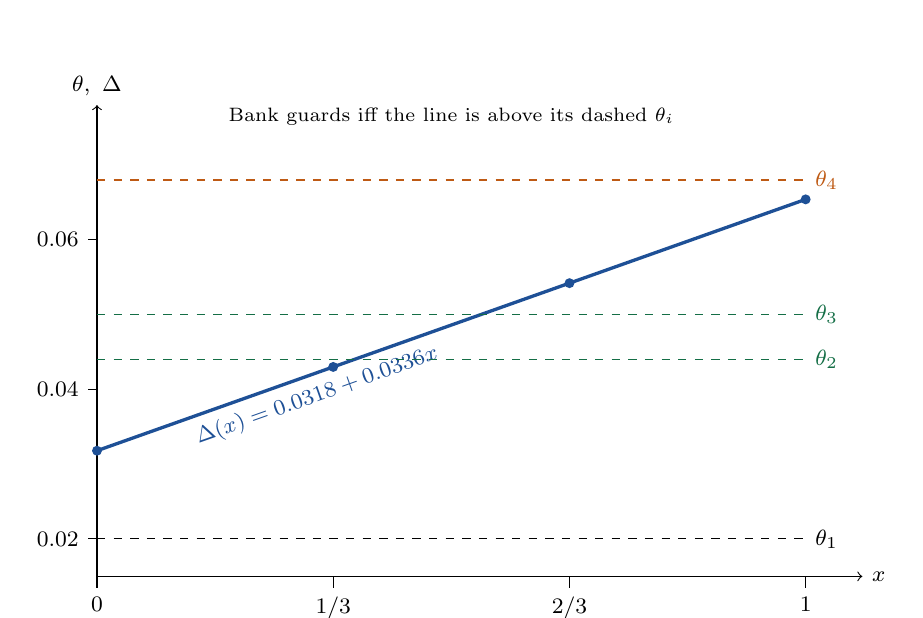
\begin{tikzpicture}[x=9cm,y=95cm,font=\footnotesize]
  \draw[->] (0,0.015) -- (1.08,0.015) node[right]{$x$};
  \draw[->] (0,0.015) -- (0,0.078) node[above]{$\theta,\ \Dl$};
  \foreach \xx/\lab in {0/0,0.3333/{1/3},0.6667/{2/3},1/1}
    \draw (\xx,0.015) -- (\xx,0.0135) node[below]{$\lab$};
  \foreach \yy in {0.02,0.04,0.06}
    \draw (0,\yy) -- (-0.012,\yy) node[left]{\yy};
  \draw[very thick,src] (0,0.0318) -- (1,0.0654) node[pos=0.3,below,sloped]{$\Dl(x)=0.0318+0.0336x$};
  \foreach \xx/\yy in {0/0.0318,0.3333/0.0430,0.6667/0.0542,1/0.0654}
    \fill[src] (\xx,\yy) circle (1.8pt);
  \foreach \t/\n/\c in {0.020/1/black,0.044/2/ans,0.050/3/ans,0.068/4/warn}{
    \draw[dashed,\c] (0,\t) -- (1.0,\t) node[right]{$\theta_\n$};}
  \node[font=\scriptsize,align=left] at (0.5,0.0765) {Bank guards iff the line is above its dashed $\theta_i$};
\end{tikzpicture}
\caption{\ours{} Guard premium $\Dl(x)$ (estimates of \S3) against the cost thresholds $\theta_i$ of the four-bank example of \S6
($x=k/3$ guarded neighbours); same logic as the paper's Figure 1 (p.\ 550), where the premium is plotted over the number of guards.
Bank 1 always guards; bank 4 guards only when $\Dl(1)$ exceeds $\theta_4$, and here it does not ($0.0654<0.068$).}
\end{figure}

%--------------------------------------------------------------------------------------------
\section{$N$ banks: ordering and multiplicity}

\subsection{The Lemma (ordering)}
\paper{} (the proof of Prop.\ 1 rests on it, p.\ 549). \textbf{In any equilibrium, if bank $i$ hires, every bank $j<i$ hires.}

\textbf{Proof} (ours, step by step). Suppose a profile has $G$ guarded banks, $i$ guarded and $j<i$ not. Bank $i$'s
neighbours include $G-1$ guards, and it hires, so $\Dl(G-1)\ge\theta_i$. Bank $j$'s neighbours include $G$ guards.
Since $\Dl$ is increasing, $\Dl(G)\ge\Dl(G-1)\ge\theta_i\ge\theta_j$, so $j$ weakly prefers to hire (strictly when $\Dl$ rises strictly and $\theta_j<\theta_i$); ignoring ties the profile is not an
equilibrium. $\square$ The script checks it on 300 random five-bank markets.

\subsection{Proposition 1 and the intuition}
By the Lemma every equilibrium is ``the first $e$ banks guard'', so an equilibrium is pinned down by its
marginal bank $e$. \paper{} \textbf{Prop.\ 1} (p.\ 549): (a) with no displacement ($\Dl$ constant) there is a unique
equilibrium, $e_0$ banks, $e_0$ the number with $\theta_i<\Dl(0)$; (b) with displacement an equilibrium with $e$
guards exists iff $\theta_e<\Dl(e-1)$ and $\theta_{e+1}\ge\Dl(e)$ (the last guard wants its guard, the first non-guard
does not want one); (c) such $e$ may be multiple, and then fewer and more banks may hire. \textbf{Intuition} (paper,
p.\ 549, Fig.\ 1 on p.\ 550): without displacement the premium is a flat line and each bank compares its $\theta$ with it; with
displacement the line slopes up, and banks that sit between $\Dl(e)$ and $\Dl(e+1)$ (similar $\theta$) can be
pulled in or out by the others: a coordination game among them.

\subsection{Proposition 3 and the paper's numbers}
\paper{} \textbf{Prop.\ 3} (complete coordination, p.\ 550): (a) if $\Dl(0)<\theta_1$ then ``no guard'' is an equilibrium; (b) if
$\Dl(1)>\theta_N$ (the paper writes $\Dl(N)$; all other banks guarded) then ``all guard'' is an equilibrium. Both
hold when banks are similar, deterrence is small and displacement is large. With $c$ equal across banks,
(a) requires every bank's $L$ below $c/\Dl(0)$ and (b) requires every bank's $L$ above $c/\Dl(1)$ (the paper's
sentence on p.\ 557 that ``some bank'' exceeds the cutoff is looser than the proposition).

\textbf{Numbers (p.\ 557).} The paper reports an all-guard equilibrium for $L>$\ \eur662{,}000 and a no-guard
equilibrium for $L<$\ \eur1.37 million, ``assuming an annual cost of 40{,}000 euros''. \ours{} \textbf{Discrepancy.}
With $c=40{,}000$ and the baseline estimates of \S3 we get $40{,}000/0.0318=1{,}257{,}862$ and $40{,}000/0.0654=611{,}621$,
not 1.37M and 662k. The paper's figures reproduce with $c=44{,}000$ and Table 4 col.\ 2 ($\beta_1=-0.0321$,
$\beta_3=-0.0343$): $44{,}000/0.0321=1{,}370{,}717$ and $44{,}000/0.0664=662{,}651$. Footnote 24 (p.\ 557) says the
yearly guard cost (\eur24.27 per hour, 7 hours, 5 days) ``is close to 44,000 euros'', so the text appears to quote 40,000 while the
computation used 44,000. The conclusion does not change: even with $c=44{,}000$ and the baseline we get 1,383,648 and 672,783.
We use $c=40{,}000$ as stated, so that every number below can be re-derived from the paper's text.

%--------------------------------------------------------------------------------------------
\section{A four-bank example}

\ours{} Four banks, $c=40{,}000$ each, with
$\theta=(0.020,\ 0.044,\ 0.050,\ 0.068)$, i.e.\ $L_1,\dots,L_4=$ 2,000,000; 909,091; 800,000; 588,235. A bank's neighbours are
the other three, $x=k/3$ for $k$ guarded others, so
\[
  \Dl(0),\Dl(1/3),\Dl(2/3),\Dl(1)=0.0318,\ 0.0430,\ 0.0542,\ 0.0654 .
\]

\subsection{Equilibria, step by step}
By the Lemma only the profiles $\{\},\{1\},\{1,2\},\{1,2,3\},\{1,2,3,4\}$ can be equilibria. Test each ($i$ inside needs
$\Dl\bigl((e-1)/3\bigr)>\theta_e$ for the last guard; the first outsider needs $\Dl(e/3)\le\theta_{e+1}$):
\begin{itemize}
  \item $\{\}$: bank 1 gains from a guard, $0.0318>0.020$. Not an equilibrium.
  \item $\{1\}$: bank 1 keeps its guard; bank 2 faces one guarded neighbour and would not hire, $0.0430<0.044$. Equilibrium.
  \item $\{1,2\}$: bank 2 has one guarded neighbour, $0.0430<0.044$, so it fires. Not an equilibrium.
  \item $\{1,2,3\}$: bank 3 sees two guards, $0.0542>0.050$; bank 4 would see three, $0.0654<0.068$. Equilibrium.
  \item $\{1,2,3,4\}$: bank 4 sees three guards, $0.0654<0.068$: it fires. Not an equilibrium.
\end{itemize}
The pure equilibria are $\{1\}$ and $\{1,2,3\}$ (the script enumerates all 16 profiles and finds exactly these).
Total expected cost (banks' losses plus guards): $\{1\}$ 290,154; $\{1,2,3\}$ 271,510; all four 252,393 (the
\textbf{social optimum}); nobody 300,813. The optimum is \emph{not} an equilibrium: bank 4's cost at all four is
52,647, but it falls to 51,118 if it fires (it gains 1,529).

\subsection{Policy: ban, requirement or subsidy}
\begin{itemize}
  \item \textbf{Ban} (all zero): 300,813, worse than either equilibrium.
  \item \textbf{Requirement} (all four): 252,393. A saving of 37,762 against $\{1\}$ and 19,118 against $\{1,2,3\}$. Bank 4 pays 1,529 more than if it were free to fire
        (52,647 against 51,118); the other banks gain more than that.
  \item \textbf{Subsidy $s$ per guard} (cost $c-s$): bank 4 is indifferent at all four when $s=c-\Dl(1)L_4=1{,}529.4$; for
        $s=1{,}600$ the unique equilibrium is all four (the script enumerates). The bill is $4\times1{,}600=6{,}400$ a year, a transfer in
        social cost.
\end{itemize}
\paper{} \textbf{Price instruments are ill suited} (p.\ 550): a tax shifts all $\theta_i$ down (to the left) \emph{strengthening} the first condition
of Prop.\ 3 (a no-guard equilibrium), \emph{weakening} the second, and only changes dispersion through $L_i$; a subsidy
can tip a market only if it moves the least-exposed bank across $\Dl(1)$. Quantity regulation, requiring or restricting guards,
removes the coordination problem by forcing a profile.

\textbf{Why the example is an exception.} \ours{} Here $\theta_4=0.068$ is only $0.0026$ above $\Dl(1)=0.0654$, a gap of 1,529 on a 40,000
cost (3.8\%). A small subsidy tips it. When the least-exposed bank is far from the threshold, the uniform subsidy needed
for it ($c-\Dl(1)L_N$) is paid to every bank, including those that would hire anyway, and quickly exceeds the benefit.

\subsection{A Figure-1-style example}
\ours{} The paper's Figure 1 (p.\ 550) shows a market with multiple equilibria and a coordination game between banks 3 and 4. Our numbers,
chosen to give the same pattern (we do not take them from the paper): $\theta=(0.025,0.035,0.058,0.060)$ gives the pure equilibria $\{1,2\}$ and $\{1,2,3,4\}$, and the
social optimum is all four. Banks 3 and 4 have $\theta$ between $\Dl(2/3)=0.0542$ and $\Dl(1)=0.0654$: each guards if and only if the other does.

%--------------------------------------------------------------------------------------------
\section{Lecture 5: the repeated game}

\ours{} \emph{This whole section is our extension; the paper's model is static.} The panel 2000--2009 is a finitely repeated game with $T=10$
yearly rounds. Notation follows Lecture 5: stage game with payoffs $u_i=-\text{cost}$, discount factor $\delta$, finite-horizon payoff
$u_i^1+\delta u_i^2+\dots$, normalized $(1-\delta)\sum\delta^{t-1}u_i^t$ in the infinite horizon.

\subsection{Any sequence of stage Nash equilibria is an SPE}
\textbf{Claim.} Let $a^1,\dots,a^T$ be stage-game Nash equilibria, and let each bank play $a_i^t$ at date $t$ whatever the history. This is an SPE.

\textbf{Proof by the one-stage deviation principle} (Lecture 5; Tadelis Ch.\ 9--10). A profile is an SPE of a finite game iff no player
gains from deviating at a single history and then following the strategy. Take any history $h^t$. If bank $i$ deviates at $t$, its stage payoff is
$u_i(a_i',a_{-i}^t)\le u_i(a^t)$ because $a^t$ is a stage NE; its continuation is unchanged because future play does not
depend on the history. So the one-stage deviation is not profitable. $\square$

\textbf{Unraveling.} In the last period $T$ some stage NE must be played after every history. If the stage game had a unique equilibrium, backward induction would give a unique SPE,
repeating it. Here there are at least two pure equilibria ($\{1\}$ and $\{1,2,3\}$) and one mixed, which gives room for carrots and sticks.

\subsection{Carrot and stick with two periods}
Play all four in $t=1$ (not a stage NE). In $t=2$, play $\{1\}$ if bank 4 complied in $t=1$ (the carrot) and $\{1,2,3\}$ if any bank deviated (the stick); both are stage
NE. Bank 4's stage costs: all four 52,647; $\{1,2,3\}$ 51,118; $\{1\}$ 44,490.

\textbf{One-stage deviation check for bank 4 at $t=1$} (cost with discounting, $c^1+\delta c^2$):
\[
  \begin{aligned}
  52{,}647+\delta\cdot44{,}490 &\le 51{,}118+\delta\cdot51{,}118\\
  \iff \delta\,(51{,}118-44{,}490)&\ge 52{,}647-51{,}118\\
  \iff \delta&\ge\frac{1{,}529}{6{,}628}=0.2307 .\end{aligned}
\]
Banks 1--3 at $t=1$: firing raises their $t=1$ cost by 90,800, 19,455 and 12,320, and changes their $t=2$ cost by $-22{,}267$, $-4{,}152$ and $+1{,}147$ (the stick
$\{1,2,3\}$ against the carrot $\{1\}$), so firing is unprofitable for every $\delta\in[0,1]$. At $t=2$ everyone plays a stage NE. By the one-stage deviation principle the
profile is an SPE iff $\delta\ge0.2307$.

\textbf{The carrot is fewer guards around you.} Bank 4 is the unguarded bank. What it values is \emph{fewer guards nearby}, because displacement is what makes robberies fall on it;
the carrot $\{1\}$ (44,490) is the equilibrium in which banks 2 and 3 have fired. The stick $\{1,2,3\}$ is the equilibrium in which bank 4 is the lone unguarded bank facing three guards (51,118).
Compliance means \emph{guarding}, which only pays because of the future. The structure echoes the Lecture 5 example: the stick is itself a Nash equilibrium, so it is credible.

With $T=10$ the same logic applies to the last two rounds ($t=9$). We do not claim that cooperation can be sustained earlier: this particular stick fails earlier (once bank 4 has deviated and the market switches to $\{1,2,3\}$, bank 4 saves 1,529 in every later period before $T$, whereas its loss comes only at $T$).

\subsection{Why Nash reversion cannot sustain all four forever}
Infinite horizon with normalized payoffs: grim trigger playing all four until someone deviates and then a stage NE forever. Bank 4's deviation gives 51,118 now and at most 51,118 later
in either stage NE ($\{1\}$ 44,490; $\{1,2,3\}$ 51,118), against 52,647 for compliance in every period. Since
$(1-\delta)\,51{,}118+\delta\,v<52{,}647$ for $v\in\{44{,}490,\ 51{,}118\}$ and every $\delta\in[0,1)$, deviation always pays. \textbf{Both stage NE are cheaper for bank 4 than the cooperative profile,}
so the punishment is no punishment: Nash reversion cannot sustain the all-four profile whatever $\delta$ is. This contrasts with the Lecture 5 homework on tacit collusion, where the stage NE profits are
lower than the collusive ones and a threshold $\delta^*<1$ exists.

\subsection{Policy reading and the evidence}
\begin{itemize}
  \item \ours{} \textbf{Quantity regulation versus repetition.} Sustaining the good profile through repetition needs the right stage NE to be less attractive than compliance; here one cannot rely on it, which fits \paper{}'s case for requirements (p.\ 550).
  \item \ours{} \textbf{A coordination device.} The Italian Banking Association (ABI) collects the census used in the paper (p.\ 550); a body like it could announce a ``guard everywhere'' standard
        as a focal point. This is our suggestion, not the paper's.
  \item \paper{} \textbf{Coordination over time} (Figs.\ 4--5, pp.\ 552--553): the share of neighbouring bank pairs that make the same guard decision rises over time. Among pairs with at least one guard, in 2000
        over 40\% have both guarded, while about 20\% would if hiring were random; a persistent 20-point gap, ``suggestive, though not dispositive, of coordinated behavior'' (p.\ 552).
  \item \paper{} \textbf{Firings outnumber hirings} (Fig.\ 3, p.\ 552), ``consistent with banks trying to disinvest in security guards''. \ours{} In game terms: with strategic complements, a few firings
        push the remaining banks toward the low-guard equilibrium.
\end{itemize}

%--------------------------------------------------------------------------------------------
\section{Observability}

\paper{} Guards are \emph{visible} to robbers (p.\ 548; the conclusion speaks of ``highly visible private security guards'', p.\ 561). Visibility is what lets a robber condition on $g$ and thus makes displacement possible.
The paper contrasts this with Ayres and Levitt (1998): car-tracking devices (LoJack) that thieves \emph{cannot observe} reduce thefts across the board, and with Gonzalez-Navarro (2013) on observable devices in Mexico, where protected cars
are less likely to be stolen but thieves turn to unprotected cars (p.\ 548).

\ours{} \textbf{Game reading.} If protection is unobservable the robber cannot direct his attempts toward unprotected targets. Each protected bank then makes \emph{every} bank's expected attempt less likely to succeed,
$\partial p/\partial g_{-i}<0$: a positive externality. The guard premium falls in others' guards, the game turns into one of strategic substitutes (free riding: let the neighbour pay), and the equilibrium has too little
protection. With observable guards the sign flips ($\partial p/\partial g_{-i}>0$ for unguarded banks), the game has strategic complements and the problem is coordination and over-investment is possible. This is a qualitative
statement; neither the paper nor the script models the unobservable case.

\textbf{Link to Lecture 4.} The Brexit lesson was that a commitment (preparation) works only when the other player observes it: observability matters. Here observability is what turns a private security decision into a
signal that robbers best-respond to, i.e.\ it creates the externality.

%--------------------------------------------------------------------------------------------
\section{The empirics read through game theory}

\paper{} Why the naive regression is biased (pp.\ 547, 553): regress robberies at bank $i$ on $g_i$ and $g_{-i}$.
\begin{itemize}
  \item \textbf{Equilibrium.} Hiring responds to crime propensity ($\theta_i$ and $L_i$ are unobserved).
  \item \textbf{Simultaneity.} Eq.\ (5) makes bank $i$'s hiring a function of $g_{-i}$, and the neighbours' hiring a function of $g_i$: best responses, hence the unobserved factors in $L_{-i}$ and $p_{-i}$ also enter
        (p.\ 553).
  \item \textbf{Manski's reflection problem.} In Manski's language (1993) the displacement effects $\beta_2,\beta_3$ correspond to \emph{correlated effects}: neighbours choose alike because they share an environment, which
        is hard to separate from the causal effect of neighbours' guards (p.\ 553).
\end{itemize}
\paper{} \textbf{Strategy.} The own-deterrence effect $\beta_1$ should not depend on the market's size, whereas the endogeneity does. Estimating $\beta_1$ with market fixed effects in successively smaller markets removes the
common factors: the estimate moves from $-0.0043$ with no fixed effects to $-0.0441$ at the 5\,km market (Table 2, p.\ 554), about ten times larger. Displacement is then estimated from how neighbours' guards shift risk within
the 500\,m market (Tables 3--4). We take the paper's results as given.

%--------------------------------------------------------------------------------------------
\section{Limits}
\begin{itemize}
  \item \textbf{Functional form.} The linear $p$ and the share $x$ are the regression's; the sampling uncertainty of $\beta_1,\beta_2,\beta_3$ is ignored here, and the thresholds scale one-for-one with $c$ (see the 44,000 discrepancy).
  \item \textbf{Unobserved $c_i,L_i$.} The paper has no data on $c_i,L_i$ (p.\ 557); our four-bank example is illustrative, not estimated.
  \item \textbf{Robbers are not players.} Displacement is built into $p$; robbers' strategic response to policy is not modelled.
  \item \textbf{Static game, simple repeated game.} The Lecture 5 section is ours: two periods, a single bank's incentive in a stylized example. Hirings are costly to reverse in practice and guards last more than a year.
  \item \textbf{Equilibria.} Pure equilibria are enumerated; mixed equilibria are derived only for $N=2$. Welfare ignores customers, employees and police.
  \item \textbf{Transfers.} A subsidy is treated as a transfer; its financing is ignored.
\end{itemize}

%--------------------------------------------------------------------------------------------
\section{Discussion questions}

\textbf{Q1. In the four-bank example the total cost is lowest at all four (252,393) and higher at $\{1\}$ (290,154). Why is $\{1\}$ an equilibrium?}
\answer{Total cost is not each bank's own cost. At $\{1\}$ bank 2 faces one guarded neighbour: $\Dl(1/3)=0.0430<\theta_2=0.044$, so a guard does not pay unless banks 3 and 4 guard too. Each bank's best response rises with the others'
guards, so a profile with few guards is self-confirming: strategic complements.}

\textbf{Q2. In the two-bank game at $L=700{,}000$, $GG$ is an equilibrium. Is it good?}
\answer{$GG$ is an equilibrium ($\Dl(1)=0.0654>\theta=0.0571$) but costs 55.05 per bank against 49.0 at $NN$ (total 110.1 against 98.0). It is Pareto dominated: too many guards (Prop.\ 2).
A restriction on guards would help, whereas at $L=10^6$ a requirement would.}

\textbf{Q3. Why can the carrot and stick sustain all four but grim trigger cannot?}
\answer{Grim trigger punishes with a stage NE forever, but both stage NE (44,490 and 51,118) are cheaper for bank 4 than all four (52,647), so deviating never hurts. With two stage NE the future can be made to depend on
bank 4's behaviour: $\{1\}$ if it complies, $\{1,2,3\}$ if it does not. The 6,628 difference, weighted by $\delta$, must exceed the 1,529 short-run gain: $\delta\ge0.2307$.}

\textbf{Q4. How would the game change if guards were invisible?}
\answer{Robbers could not condition on guards, so there would be no displacement: $\partial p/\partial g_{-i}\le0$, the premium falls with neighbours' guards and the game becomes strategic substitutes (free riding),
as in LoJack (Ayres--Levitt, p.\ 548). Compare Lecture 4: observability changes the equilibrium.}

\textbf{Q5. A subsidy of 1,600 fixes the four-bank market. Why would a policymaker still prefer a requirement in many markets?}
\answer{The subsidy works only because $\theta_4$ is close to $\Dl(1)$. The uniform subsidy needed equals $c-\Dl(1)L_N$ for the least-exposed bank and goes to all banks; the more dispersed the $\theta$'s, the larger it is.
A requirement forces the profile at no price (paper, p.\ 550), though it needs information on which profile is efficient.}

\textbf{Q6. Is the 1.37M/662k discrepancy important?}
\answer{It shows that the cutoffs scale with $c$: $c=44{,}000$ and Table 4 col.\ 2 give the paper's 1.37M and 662k; $c=40{,}000$ and the baseline give 1,257,862 and 611,621. The qualitative result,
a wide range of $L$ where both equilibria exist, is unchanged (even $c=44{,}000$ with the baseline gives 1,383,648 and 672,783).}

\end{document}
